\section{Reproducibility in Scientific Workflows}
\label{sec:reproducibility}

In this section, we introduce the tools used for the instantiation and evaluation 
of the aforementioned semantic models. We first describe the Pegasus Workflow 
Management System (WMS)~\cite{Deelman-FGCS-2014}, which is used as \rev{the }
workflow engine, and then a set of reproducibility tools for semantic annotations and 
experiment management.


% subsection
\subsection{Scientific Workflow Execution}

The Pegasus WMS can manage workflows comprised of millions of tasks, recording data 
about their execution and intermediate results. In Pegasus, workflows are described as 
abstract workflows, that is, they do not contain resource information, or the physical locations of 
data and executables. Workflows are described as directed acyclic graphs (DAGs), where 
nodes represent individual computational tasks and the edges represent data and control 
dependencies between tasks. The abstract workflow description is represented as a DAX 
(DAG in XML), capturing all the tasks that perform computations, the execution order of these 
tasks, and for each task the required inputs, expected outputs, and the arguments with which 
the task should be invoked. 

During a workflow execution, Pegasus translates an abstract workflow into an 
executable workflow, determining the executables, data, and computational resources 
required for the execution. Pegasus maps executables to their installation paths or to a 
repository of stageable binaries defined in a Transformation Catalog (TC). A workflow 
execution includes data management, monitoring, and failure handling. Individual workflow 
tasks are managed by a task scheduler (HTCondor~\cite{condor}), which supervises their 
execution on local and remote resources.


% subsection
\subsection{Reproducibility Artifacts}

To conduct the experimentation on scientific workflows reproducibility, we 
use the WICUS framework~\cite{wicus}, which comprises the semantic models described 
in Section~\ref{sec:semantic} and a set of tools for annotating and consuming data; and 
the PRECIP~\cite{Azarnoosh-CRC-2013} experiment management tool to manage the 
experiment. In addition, we use Vagrant~\cite{palat2012introducing}, a tool for deploying virtual
deployment environments,  to achieve local reproducibility of the experiments. 
Below, we describe each of these tools in detail.


\subsubsection{WICUS}
\label{subsec:wicus}

Besides the ontology network introduced before, a set of components have been developed around it, 
for facilitating the annotation of the resources involved in the execution of a scientific workflow. 
These tools are not fully automated yet, but represent a first step in helping users define the requirements of their 
experiments. Figure~\ref{fig:wicusflow} shows the main modules involved in the process for achieving reproducibility. 
It also describes the process of data generation and consumption. Below, we provide an overview of each of these modules:

\begin{figure}[!htb]
	\centering
	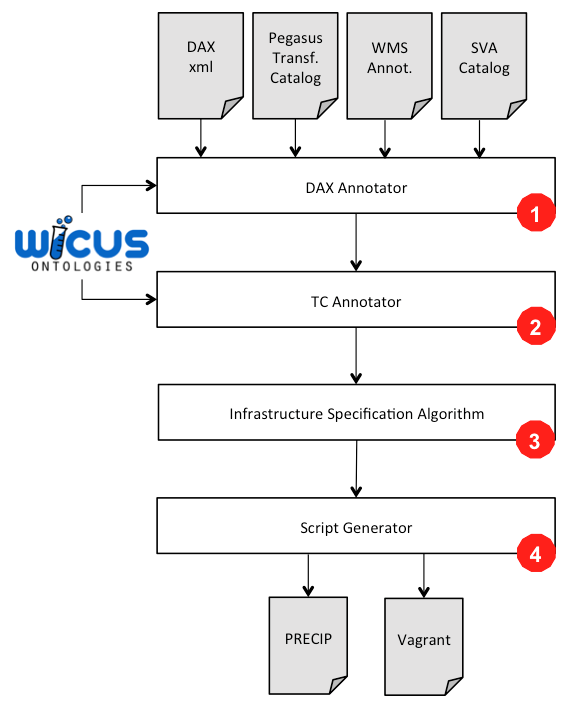
\includegraphics[width=.8\linewidth]{figures/wicusflow}
	\caption{WICUS annotation modules and flow. White boxes represent tools for semantic annotation or algorithms, and grey boxes represent files used or generated by the framework.}
	\label{fig:wicusflow}
\end{figure}

\begin{enumerate}
	\item \textbf{DAX Annotator.} This tool parses a DAX (Pegasus' workflow description) 
		and generates a set of annotations using the terms of the WICUS ontology network, 
		representing workflow transformations and the workflow infrastructure requirements.
		\rev{As a result of this process, a file containing the description of the workflow and 
		its infrastructure requirements is generated.}

%	\item \textbf{WMS Annotations.} This RDF file contains the information of the WMS component 
%		and its dependencies. This information is added to the \emph{Software Components 
%		Catalog}.

	\item \textbf{Transformation Catalog Annotator.} This tool parses the Pegasus Transformation 
		Catalog and the WMS annotations file, to generate two set of annotations: the \emph{Software 
		Components Catalog} file, \rev{which contains the set of annotations about 
		the binaries, dependencies, deployment plans and scripts, and the \emph{Workflow \& Configuration 
		Annotation} file, containing the configuration information for each workflow execution step, as 
		specified in the transformation catalog.}

%	\item \textbf{Software Components Catalog.} This RDF file contains the set of annotations about 
%		the binaries, dependencies, deployment plans and scripts, and configuration information of 
%		the software involved in the experiment.
%
%	\item \textbf{Workflow \& Configuration Annotation File.} This RDF file contains the same information 
%		as in 2, but enriched with the configuration information for each workflow execution step, as 
%		specified in the transformation catalog.
%
%	\item \textbf{Scientific Virtual Appliances Catalog.} This RDF file contains available \rev{SVAs}. 
%		Information about the related infrastructure providers and the VM images that compose an 
%		appliance are included in this dataset.

	\item \textbf{Infrastructure Specification Algorithm.} This process reads files 
		\rev{generated on the previous steps and generates a file containing 
		the \emph{Abstract Deployment Plan} describing the VMs to be created,
		and the software components to be deployed. This plan will be enacted 
		later using a concrete language.}
		% This decoupled approach facilitates the integrations of new enactment systems.}
		
	\item \textbf{Script Generator.} This module concretizes the abstract deployment 
		plan using the selected language (either PRECIP or Vagrant in this case) to 
		generate an executable script. New script syntaxes may be added in the future.

%	\item \textbf{Executable Script.} This script creates a PRECIP/Vagrant experiment, which runs a VM, 
%		copies the required binaries, and executes deployment scripts to set the environment for the 
%		workflow execution. It also contains the original experiment commands in order to 
%		re-execute it.
\end{enumerate}

\rev{The main entries of the WICUS process include the \emph{DAX XML} file
(DAG in XML), and the \emph{Pegasus Transformation Catalog} file, which 
contains the information about the software components required by the workflow.
It also requires the \emph{WMS Annotations} file, which describes the Pegasus 
system, and the \emph{SVA Catalog} file, which contains information about the
available computational resources. Both files are generated manually using 
the WICUS ontologies. Upon completion, the process outputs execution scripts,
%(either using PRECIP or Vagrant)
which create a VM, copy the required 
binaries, and execute the deployment scripts to set the environment for the 
workflow execution. It also contains the original experiment commands in order 
to re-execute it.}

\rev{In this work, we introduce our current use case using PRECIP and Vagrant 
as enactment systems for recreating the execution environments. Thanks to
the decoupled design of the system, additional solutions could be easily 
incorporated by extending the \emph{Script Generator} component. For instance,
the \emph{Abstract Deployment Plan} could be translated into new syntaxes to
explore new technologies such as Docker containers~\cite{Merkel2014}, or 
TOSCA templates.}
 
 
In the experimentation process (Section~\ref{sec:experiment}), we will present 
a detailed description and the applicability of each module for the target 
scientific \rev{workflow applications}.


\subsubsection{Infrastructure Specification Algorithm}

\rev{
The third step on the process for achieving reproducibility in scientific workflows 
(Figure~\ref{fig:wicusflow}) is to execute the Infrastructure Specification Algorithm 
(ISA). The algorithm retrieves the corresponding information for the 
workflow and its dependencies from the annotation datasets, and calculates the 
dependencies and compatibility between requirements and the available 
computational resources. It also considers the software already installed on the
resources to avoid unnecessary installation steps.

Listing~\ref{lst:pseudo} shows the pseudo-code of the algorithm. ISA combines 
the annotated data based on the 4 domain ontologies in order to find a suitable 
infrastructure specification that meets the requirements of the workflow. The 
algorithm retrieves and propagates the WMS requirements of the top-level 
workflow (\texttt{Workflow} domain ontology) to its related sub-workflows (as 
defined in Figure~\ref{fig:annotations}). Requirements  and software components 
are matched, and a dependency graph is built based on the relationship between 
the requirements and the component dependencies (line 13). ISA then calculates 
the intersection between the set of components installed on the SVA and the set 
of components from the dependency graph, selecting the SVA that maximizes the 
value of that intersection for each sub-workflow (line 17). Software components 
already available in the SVA are then removed from the dependency graph, as they 
do not have to be installed (line 19). To reduce the number of SVAs, we have extended
ISA to support \emph{Image Appliance} filtering. The algorithm attempts to merge 
sub-workflow requirements into a single SVA (line 21). Requirements can be merged 
if all their software components are compatible. Thus, the algorithm filters those that 
do not meet the hardware requirements specified for the workflow (lines 23--25).
Finally, ISA generates a script with the set of required instructions to instantiate, 
configure, and deploy the computational resources and software components on 
the corresponding provider (line 27). To enact support to different execution scripts, 
we introduced an intermediate phase (\emph{Abstract Deployment Plan}), which 
defines the steps and scripts to be executed, along with their configuration 
parameters. We also extended ISA to generate Vagrant scripts in addition to
PRECIP. A complete description and evaluation of the algorithm can be found 
in~\cite{wicus}.}

%\rev{In this work, we have extended ISA to support 1)~Image Appliance filtering, and 
%2) generation of Vagrant scripts. From the selected SVAs, the algorithm filters those that
%do not meet the hardware requirements specified for the workflow
%(lines 23--25). To enact support to different execution scripts, we introduced an intermediate 
%phase (\emph{Abstract Deployment Plan}), which defines the steps and scripts to be executed, 
%along with their configuration parameters.}
%ISA then translates this plan into a PRECIP or Vagrant script depending on the resultant target provider (line 27).}
          
\begin{lstlisting}[caption={Pseudo-code overview of the Infrastructure Specification Algorithm (ISA).},label={lst:pseudo},basicstyle=\footnotesize]
WorkflowRequirementsDataset.load();

SVADataset.load();

SoftwareCatalogDataset.load();

Map<Workflow,List<Requirements>> wfSwReqs = retrieveSwRequirements( WorkflowRequirementsDataset, WorkflowID );

Map<Workflow,List<Requirements>> propagatedWfSwReqs = propagateSwReqs( wfSwReqs );

List<List<List<SWComponents>>> softwareComponents = getSoftwareComponents( propagatedWfSwReqs );

Map<Requirement,D-Graph<SWComponents>> softwareComponentsDependencyGraph =    getSoftwareDependencies(softwareComponents );

List<SVA> availableSvas = getAvailableSvas(providersList);

Map<Requirements,SVA> maxCompatibilities = getCompatibilityIntersection( softwareComponentsDependencyGraph, availableSvas );

Map<Requirement,D-Graph<SWComponents>> substractedSwComponentsDepGraph =  substractSoftwareComponents( softwareComponentsDependencyGraph, maxCompatibilities );

Map<SVA, List<Requirments>>mergedSvas= mergeSubworkflows( propagatedWfSwReqs, maxCompatibilities );

Map<Workflow,List<Requirements>> wfHwReqs =  retrieveHwRequirements( WorkflowRequirementsDataset, WorkflowID );

Map<SVA, List<Requirments>>filteredSvas= getCompatibleHwImageAppliances( mergedSvas, wfHwReqs );

generateScript( filteredSvas, substractedSwComponentsDepGraph );
\end{lstlisting}



% PRECIP
\subsubsection{PRECIP}

The Pegasus Repeatable Experiments for the Cloud in Python 
(PRECIP)~\cite{Azarnoosh-CRC-2013} is a flexible experiment 
management control API for running experiments on all types of 
Clouds, including academic Clouds such as FutureGrid\footnote{http://portal.futuregrid.org} 
and the NSFCloud\footnote{http://www.chameleoncloud.org}\textsuperscript{,}\footnote{http://cloudlab.us}
(through OpenStack), and commercial Clouds such as Amazon 
EC2\footnote{http://aws.amazon.com/ec2} and Google Compute 
Engine\footnote{https://cloud.google.com/compute}. \rev{In PRECIP, 
when an instance is provisioned, the scientist can add arbitrary 
tags to that instance in order to identify and group the instances 
in the experiment. Then, future interactions can be performed by 
using the given tags}. API methods such as running remote commands, 
or copying files, all use tags to specify which instances to target. 
PRECIP does not force the scientist to use a special VM image, 
and no PRECIP components need to be pre-installed in the image. 
Scientists can use any basic Linux image and PRECIP will bootstrap 
instances using SCP and SSH commands. PRECIP provides 
functionality to run user-defined scripts on the instances to install/configure 
software and run experiments, and also manages SSH keys and 
security groups automatically.

In this work, we use PRECIP to define a script able to reproduce 
the execution environment of the former experiment, and run it on 
a Cloud platform.


% Vagrant
\subsubsection{Vagrant}

Vagrant~\cite{palat2012introducing} is an open-source and multi-platform solution for deploying 
development environments locally using virtualization. It relies on virtualization solutions such as 
Oracle VirtualBox~\cite{Watson2008} (also open-source) or  VMWare\footnote{http://www.vmware.com}, and support 
Amazon EC2-like server configurations. Since version 1.6 it also supports Docker~\cite{Merkel2014} 
containers.
Vagrant provides a set of commands and configuration files to enact and customize virtual machines
(also referred to as boxes). It allows defining the set of commands and/or scripts to be executed during 
the different stages of the booting process. Several base images are publicly available for users to 
download and customize\footnote{http://www.vagrantbox.es}. 
 
In this work, we introduce how Vagrant can be used for achieving reproducibility in a local execution
environment---usually a scientist's laptop/desktop computer. As a result, users are able to repeat and 
modify their original experiment, repurposing or improving it, which is a highly desirable goal of any 
reproducibility process. By executing Vagrant with the resultant {\it Vagrantfile} generated by the Infrastructure Specification Algorithm, 
the user will create a virtual machine on its own computer and automatically execute the workflow, 
being also able to access it and modify the environment.




